\documentclass{article}

\usepackage{datetime}
\usepackage[utf8]{inputenc}
\usepackage[margin=30mm]{geometry}
\usepackage{graphicx}

\setlength{\parskip}{\medskipamount}
\setlength{\parindent}{0pt}

\begin{document}
\title{T1: Likemannsnettverk \\ TDT4190}
\author{Kjetil Sletten, Simen Skoglund og Christian Peter}
\date{\today}
\maketitle
\section*{Oppgave 1} 
\subsection*{a)} 
Vi ville valgt likemannsnettverk. Ta for eksempel en stor fil. I en klient-tjener vil denne fila kun være tilgjengelig fra serveren og vil dermed være begrenset av linja til serveren. Brukerne som er langt bak i køen, vil kanskje avslutte og en annen vil prøve å laste ned. Dette vil resultere i en tregere nedlastning for de som fortsatt prøver å få tak i fila.  

Ved et likemannsnettverk vil den store fila bli delt opp i mindre deler, og vil dermed distribuert over forskjellige brukerne. Kostnaden ved å distribuere fila vil dermed bli mye mindre enn ved et klient-server.
\subsection*{b)} 
\emph{GUID} - Globally Unique ID, unik ID for hver node i nettverket. I et ustrukturert nettverk behandles alle nodene likt, det er jo ingen struktur på nettverket og har dermed ingenting å si om hvilken node som bearbeides.

I et strukturert nettverk må en alltid ha oversikt over hvor de forskjellige brukerene er, slik at en kan ta bruk i for eksempel Distribuert Hash Tabell. På den måten har en alltid oversikt over de forskjellige filene.
\section*{Oppgave 2} 
\subsection*{a)} 
\begin{center}
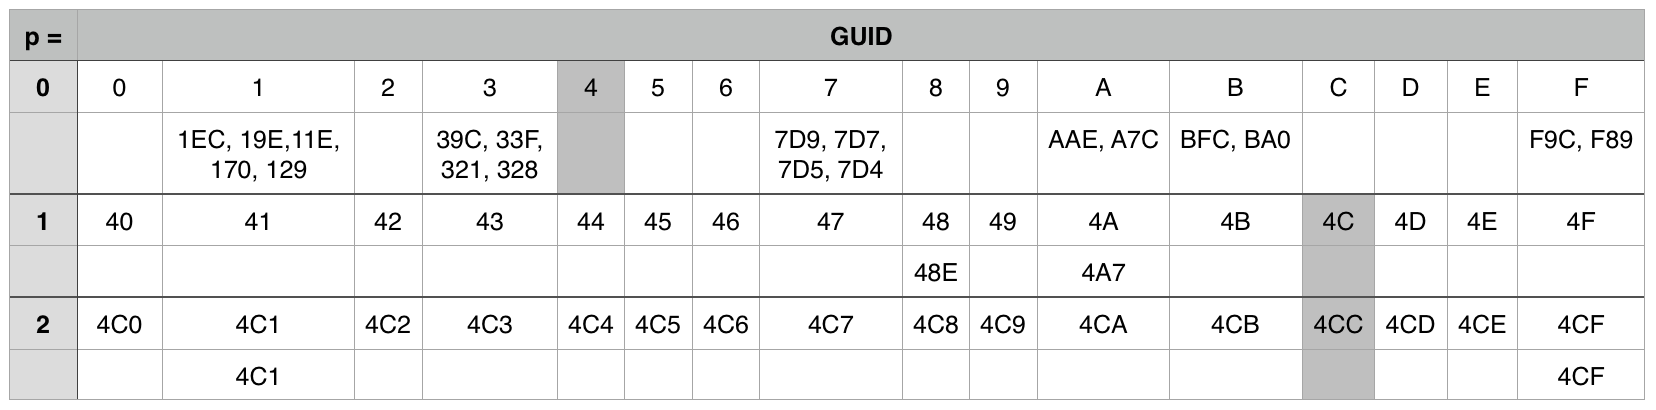
\includegraphics[scale=0.5]{Images/4CC}
\\
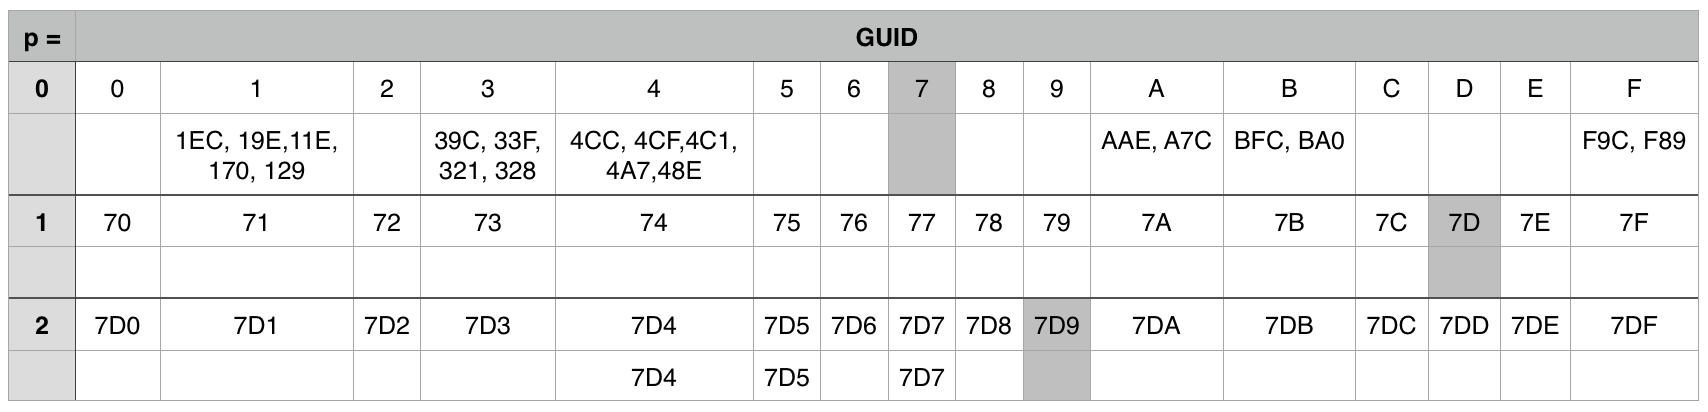
\includegraphics[scale=0.5]{Images/7D9}
\end{center}
\subsection*{b)}
Bruker pastery algoritmen fra boka side 456.

Starter på node 7D9, sjekker om destinasjonsnoden er i løvnodetabellen, det er den ikke, så går videre til neste steg. Det er å sjekke prefixlengde på 7D9 og 371 som er 0. Slår opp på rad 0 kolonne (0+3) i routingtabellen til 7D9 som er 3. Går til første node i pasterynettverket som begynner på 3. Dette er i vårt tilfelle 328 og kjører algoritmen på nytt. Sjekker om destinasjonsnoden er i løvnodetabellen til 328 noe som den er. Sender meldingen og terminerer. Prosessen er nå ferdig.
\begin{center}
	
\includegraphics[scale=0.5]{Images/Pastry}
\end{center}
\subsection*{c)}
Node X, den nye noden, har GUID 0FC. Den kontakter node A som har GUID 7D9. Node X sender en spesiell \emph{join} forespørsel til A, som gir X(GUID 0FC) som sin destinasjon. Node A sender join melding ut i Pastrynettverket. Nettverket vil så sende denne joinmeldingen til en GUID som er nærme X sin GUID, i vårt tilfelle 0FB også kalt Z. Nodene A,Z og de andre nodene som er knyttet til joinmelding utsendt fra nettverket for å komme fram til node Z, vil legge til flere steg i den vanlige Pastry routing algoritmen. 

Denne prosessen resulterer i at node X får de viktige delene av routing tabellene og løvnodetabellene fra nodene som har vært en del av join-prosessen. X kan da lage sin egen routingtabell og løvnodetabell basert på denne informasjonen. Til slutt når X har laget ferdig sin løvnodetabell og routingtabell så sender node X en melding til alle nodene i løvnodetabellen og routingtabellen, disse nodene vil da oppdaterer seg med den nye noden X(GUID 0FC). Hele denne prosessen tar O(Log(n)) tid.
\subsection*{d)}
Som oppgaven sier, vil en node miste tilkoblingen til nettverket og er dermed "død". Altså, naboene i pastry nettverket kan ikke kommunisere med den lenger. Det som må skje da er at løvnodetabellen(Kalt L) til noden som har feilet, må repareres. Det er ikke oppgitt hvilken node som oppdager feilen, men la oss si dette er node A. 

Node A må finne en node(kaller denne node Z) som fungerer i nærheten av den noden som har feilet. Den vil da be om at node Z kopierer sin løvnodetabell(Kalt L'). L' vil inneholde en sekvens av GUID'er, som delvis overlapper de i L. Her er det også en verdi som vil kunne erstatte den noden som har feilet. De andre naboene er også informert om feilen og de vil også kjøre en lignende prosess. Dette vil fungere godt, med et unntak. Hvis alle noder i samme område feiler, vil det være vanskelig å gjenopprette disse.
\end{document}